\section{Adwords}

\begin{frame}
    \frametitle{Assumptions}
	\begin{enumerate}
        \item<1-> Each bid is small compared to the corresponding budget \mbox{(i.e., $\forall (u,v) \in E: c_{u,v} \ll b_u$}).
        \invisible<1->{
            \item<1-> Each bidder has a budget of $1$.
            \item<1-> \textcolor{orange}{OPT} exhausts the budget of each bidder.
            \item<1-> Each bidder of type $i \in \{1,...,k \}$ spends exactly $\frac{i}{k}$.
            \item<1-> All non-zero bids are equal.   
        }
	\end{enumerate}
\end{frame}

\begin{frame}
    \frametitle{Landscape of Problems}
    \centering
    \begin{tikzpicture}
		\draw[very thick,orange] \orangeellipse;
		\draw[very thick,blue] \blueellipse;
		\draw[very thick,violet] \violetellipse;
		\draw[very thick,red] \redellipse;
	\end{tikzpicture}
\end{frame}

\begin{frame}
    \frametitle{GREEDY}
    \begin{algorithm}[H]
        \DontPrintSemicolon
        \caption{GREEDY}
        \When{the next vertex $v \in V$ arrives}{
            \If{all neighbors of $v$ are unavailable}{\Continue \;}
            \Else{match $v$ to that available neighbor $u \in U$ which maximizes $c_{u,v}$\;}
        }
    \end{algorithm}
\end{frame}

\begin{frame}
    \frametitle{BALANCE}
    \begin{algorithm}[H]
        \DontPrintSemicolon
        \caption{BALANCE}
        \When{the next vertex $v \in V$ arrives}{
            \If{all neighbors of $v$ are unavailable}{\Continue \;}
            \Else{match $v$ to that available neighbor $u \in U$ which has spent the \textcolor{blue}{least fraction} of its budget so far\;}
        }
    \end{algorithm}
\end{frame}

\begin{frame}
    \frametitle{Competitive Ratio}
    \begin{definition}
        In a \alert{competitive analysis}, an \textcolor{blue}{online} algorithm \textcolor{orange}{ALG} is compared to an \textcolor{blue}{optimum offline} algorithm \textcolor{orange}{OPT}.\\
        \smallskip
        Given the entire graph $G = (U,V,E)$ and the input order of $V$, $\sigma$, let \textcolor{orange}{ALG}($G, \sigma$) denote the value of the objective function attained by \textcolor{orange}{ALG}, and let \textcolor{orange}{OPT}($G, \sigma$) denote the maximum objective function value attained offline.\\
        \smallskip
        The algorithm \textcolor{orange}{ALG} is called $\alpha$-\alert{competitive} if $\frac{\text{\textcolor{orange}{ALG}}(G, \sigma)}{\text{\textcolor{orange}{OPT}}(G, \sigma)} \geq \alpha$ for all graphs $G$ and all input orders $\sigma$. The factor $\alpha$ is also called the \alert{competitive ratio} of \textcolor{orange}{ALG}.
    \end{definition}
\end{frame}

\begin{frame}
    \frametitle{Two Extreme Examples for the Adwords Problem}
    \begin{example}
        \centering
        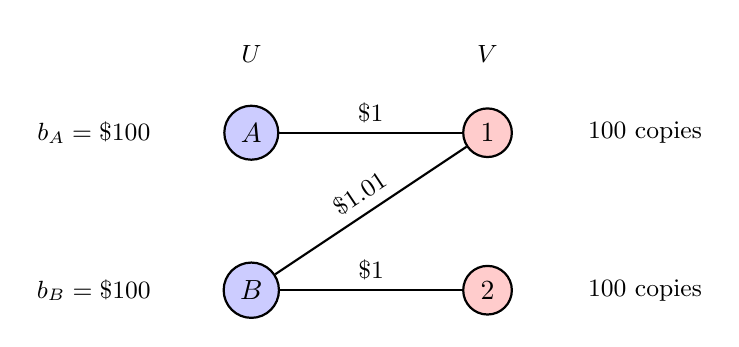
\begin{tikzpicture}
            \node[circle] at (0,3) {\small{$U$}};
            \node[draw,thick,fill=blue!20,circle] at (0,2) (A) {$A$};
            \node at (-2,2) {\small{$b_A = \$100$}};
            \node[draw,thick,fill=blue!20,circle] at (0,0) (B) {$B$};
            \node at (-2,0) {\small{$b_B = \$100$}};

            \visible<2->{
                \node[circle] at (3,3) {\small{$V$}};
                \node[draw,thick,fill=red!20,circle] at (3,2) (1) {$1$};
                \node at (5,2) {\small{$100$ copies}};
            }
            
            \visible<3->{
                \node[draw,thick,fill=red!20,circle] at (3,0) (2) {$2$};
                \node at (5,0) {\small{$100$ copies}};
            }
            
            \visible<2->{
                \draw[thick] (A) -- node[above] {\small{$\$1$}} (1);
                \draw[thick] (B) -- node[above,sloped] {\small{$\$1.01$}} (1);
            }
            
            \visible<3->{\draw[thick] (B) -- node[above] {\small{$\$1$}} (2);}
        \end{tikzpicture}
        \flushleft
        \visible<4->{
            \textcolor{orange}{GREEDY} achieves a ratio of $\frac{1}{2}$.\\
            \textcolor{orange}{BALANCE} achieves a ratio of $\frac{3}{4}$.
        }
    \end{example}
\end{frame}

\begin{frame}
    \frametitle{Two Extreme Examples for the Adwords Problem}
    \begin{example}
        \centering
        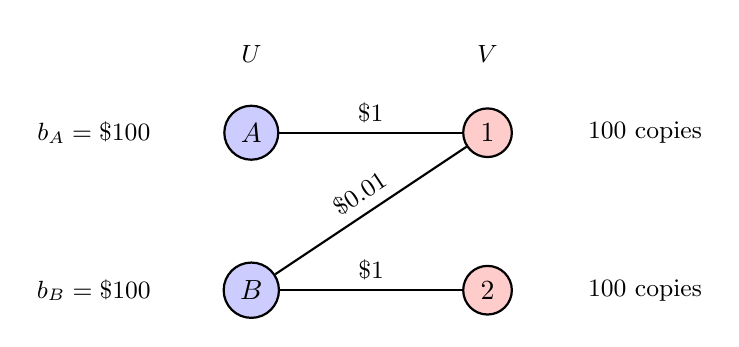
\begin{tikzpicture}
            \node[circle] at (0,3) {\small{$U$}};
            \node[draw,thick,fill=blue!20,circle] at (0,2) (A) {$A$};
            \node at (-2,2) {\small{$b_A = \$100$}};
            \node[draw,thick,fill=blue!20,circle] at (0,0) (B) {$B$};
            \node at (-2,0) {\small{$b_B = \$100$}};
    
            \node[circle] at (3,3) {\small{$V$}};
            \node[draw,thick,fill=red!20,circle] at (3,2) (1) {$1$};
            \node at (5,2) {\small{$100$ copies}};
            \node[draw,thick,fill=red!20,circle] at (3,0) (2) {$2$};
            \node at (5,0) {\small{$100$ copies}};
    
            \draw[thick] (A) -- node[above] {\small{$\$1$}} (1);
            \draw[thick] (B) -- node[above,sloped] {\small{$\$0.01$}} (1);
            \draw[thick] (B) -- node[above] {\small{$\$1$}} (2);
        \end{tikzpicture}
        \flushleft
        \visible<2->{
            \textcolor{orange}{GREEDY} achieves a ratio of $1$.\\
            \textcolor{orange}{BALANCE} achieves a ratio of $\frac{1}{2}$.
        }
    \end{example}
\end{frame}

\begin{frame}
    \frametitle{Online $b$-Matching Problem}
    \begin{block}{Online $b$-Matching Problem}
        The Online $b$-Matching problem is the special case of the Adwords problem in which
        \begin{itemize}
            \item<1-> each \textcolor{blue}{budget} is equal to $b \in \mathbb{N}$
            \item<1-> each non-zero \textcolor{blue}{bid} is equal to $1$
        \end{itemize}
    \end{block}
\end{frame}

\begin{frame}
    \frametitle{Landscape of Problems}
    \centering
    \begin{tikzpicture}
        \draw[very thick,orange] \orangeellipse;
        \draw[very thick,blue] \blueellipse;
		\draw[very thick,violet] \violetellipse;
		\draw[very thick,green!70!black] \greenellipse;
		\draw[very thick,red] \redellipse;
	\end{tikzpicture}
\end{frame}

\begin{frame}
    \frametitle{MSVV}
    \begin{algorithm}[H]
        \DontPrintSemicolon
        \caption{MSVV}
        \When{the next vertex $v \in V$ arrives}{
            \If{all neighbors of $v$ are unavailable}{\Continue \;}
            \Else{match $v$ to that available neighbor $u \in U$ which maximizes $c_{u,v} \psi\left(\frac{s_u}{b_u} \right)$,\\
            where $s_u$ is the amount of $u$'s budget spent so far, and $\psi(x) = 1 - e^{x - 1}$\;}
        }
    \end{algorithm}
    \smallskip
    If the \textcolor{blue}{budgets} are all infinity, then \textcolor{orange}{MSVV} becomes \textcolor{orange}{GREEDY}.\\
    If the \textcolor{blue}{bids} are all equal, then \textcolor{orange}{MSVV} becomes \textcolor{orange}{BALANCE}.
\end{frame}